\chapter{Quantile regression}
\label{chap:quantreg}

\section{Introduction}
\label{sec:rq-intro}

FIXME

This note documents the state of play with quantile regression in
\textsf{gretl} as of May, 2008, in CVS and the Windows snapshot.  This
functionality borrows from the \texttt{quantreg} package for
\textsf{R}, version 4.17.  The core of the \texttt{quantreg} package
is composed of Fortran code written by Roger Koenker; this is
accompanied by various driver and auxiliary functions written in the
\textsf{R} language by Koenker amd Michael Maechler.  The latter
functions have been re-worked in C for \textsf{gretl}.

\section{Basic syntax}

The basic invocation of quantile regression is

\vspace{1em}
\noindent
\qquad \texttt{quantreg} \textsl{tau} \textsl{reglist}
\vspace{1em}

where

\begin{itemize}
\item \textsl{reglist} is a standard \textsf{gretl} regression list
  (dependent variable followed by regressors, including the constant
  if an intercept is wanted); and
\item \textsl{tau} is the desired conditional quantile, in the range
  0.01 to 0.99, given either as a numerical value or the name of a
  pre-defined scalar variable (but see below for a further option).
\end{itemize}

Estimation is via the Frisch--Newton interior point solver (Portnoy
and Koenker, 1997), which is substantially faster than the
``traditional'' Barrodale--Roberts (1974) simplex approach for large
problems.

By default, standard errors are computed according to the asymptotic
formula given by Koenker and Bassett (1978).  Alternatively, if the
\verb|--robust| option is given, we use the sandwich estimator
developed in Koenker and Zhao (1994).\footnote{These correspond to the
  \texttt{iid} and \texttt{nid} options in \textsf{R}'s
  \texttt{quantreg} package, respectively.}

\section{Confidence intervals}

An option \verb|--intervals| is available.  When this is given we
print confidence intervals for the parameter estimates instead of
standard errors.  These intervals are computed using the rank
inversion method and in general they are asymmetrical about the point
estimates.  The specifics of the calculation are inflected by the
\verb|--robust| option: without this, the intervals are computed on
the assumption of IID errors (Koenker, 1994); with it, they use the
heteroskedasticity-robust estimator developed by Koenker and Machado
(1999).

By default, 90 percent intervals are produced.  You can change this by
appending a confidence value (expressed as a decimal fraction) to the
intervals option, as in

\vspace{1em}
\noindent
\qquad \texttt{quantreg} \textsl{tau} \textsl{reglist} \verb|--intervals=.95|
\vspace{1em}

When the confidence intervals option is selected, the parameter
estimates are calculated via Barrodale--Roberts.  This is simply
because Roger Koenker's Frisch--Newton code does not currently support
the calculation of confidence intervals.

\section{Multiple quantiles}

There's a further option: you can give \textsl{tau} as a
matrix --- either the name of a predefined matrix or in numerical form,
as in \verb+{.05, .25, .5, .75, .95}+.  This implies the
\verb|--intervals| option.  We estimate the given model for all
the $\tau$ values and print the results in a special form:

{\small
\begin{verbatim}
Model 1: Quantile estimates using the 235 observations 1-235
Dependent variable: foodexp
With 90 percent confidence intervals

      VARIABLE      TAU    COEFFICIENT      LOWER        UPPER

  const             0.05      124.880      98.3021      130.517
                    0.25      95.4835      73.7861      120.098
                    0.50      81.4822      53.2592      114.012
                    0.75      62.3966      32.7449      107.314
                    0.95      64.1040      46.2649      83.5790

  income            0.05     0.343361     0.343327     0.389750
                    0.25     0.474103     0.420330     0.494329
                    0.50     0.560181     0.487022     0.601989
                    0.75     0.644014     0.580155     0.690413
                    0.95     0.709069     0.673900     0.734441
\end{verbatim}
}

The \app{gretl} GUI has an entry for Quantile Regression (under
\textsf{/Model/Robust estimation}), and you can select multiple
quantiles there too.  In that context, just give space-separated
numerical values (as per the predefined options).  When you estimate a
model in this way most of the standard menu items in the model window
are disabled, but one extra item is available --- graphs showing the
$\tau$ sequence for a given coefficient in comparison with the OLS
coefficient.  An example is shown in Figure~\ref{fig:tau}.

\begin{figure}
  \centering
  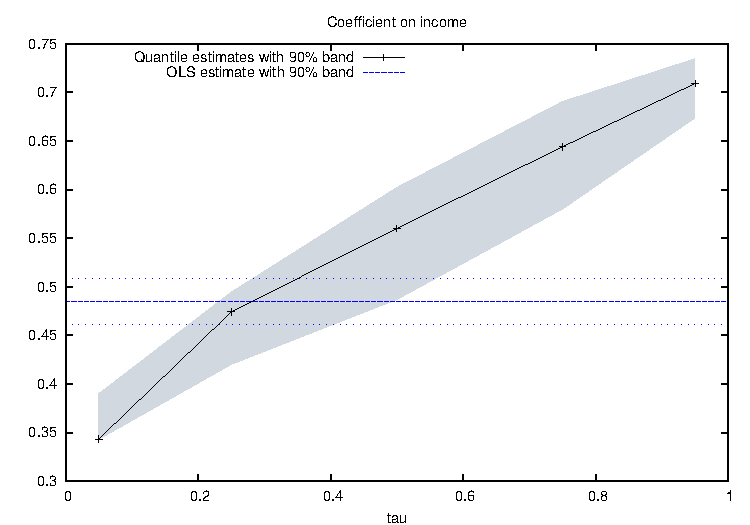
\includegraphics[scale=.8]{figures/tau-sequence}
  \caption{The income coefficient in Engel's data}
  \label{fig:tau}
\end{figure}

